\chapter{Kapitel 1: Charakter}
\section{Charakter-Erstellung}
\subsection{Volk wählen}
Wähle ein Volk und schreibe die folgenden Werte, Volksmerkmale und Informationen (teilweise auch aus aus den Beschreibungen im PH) auf:
\begin{itemize}
  \item erhöhung der Attributwerte
  \item Alter
  \item Gesinnung
  \item Größe
  \item Bewegungsrate
  \item Sprachen
\end{itemize}

\subsection{Klasse wählen}
Wähle eine Klasse und schreibe die folgenden Werte und Informationen aus den Beschreibungen im PH auf:
\begin{itemize}
  \item Vorzüge/Klassenmerkmale
  \item Übungsbonus
  \item Trefferwürfel
    \subitem \textit{(Völkerbonus:siehe Tabelle PH S.12)}
\end{itemize}

\subsection{Stufen}
Einigt euch auf eine Stufe eurer Charaktere. \\
\textit{Empfohlen: Stufe 1, 0 EP}\\
\textit{für die Stufentabelle: PH S. 15}

\subsection{Attributwerte}
Es Existieren folgende Attributwerte die bestimmt werden müssen.
\begin{itemize}
  \item Stärke
  \item Geschwindigkeit
  \item Konstitution
  \item Intelligenz
  \item Weisheit
  \item Charisma
\end{itemize}
Dafür gibt es zwei Varianten:

\subsubsection{Generierung}
\subsubsection{\small Schritt 1}
Wiederhole diesen Vorgang 6 Mal:
\begin{itemize}
  \item Würfel vier mal w6
  \item nehme die höchsten drei Werte
  \item addiere sie
  \item schreibe sie auf
\end{itemize}
Du kannst auch alternativ die Werte \\ \textit{15, 14, 13, 12, 10, 8} \\ verwenden, wenn du Zeit sparen möchtest.
\subsubsection{\small Schritt 2}
Weise nun jeden Wert einem Attribut zu.

\subsubsection{\small Schritt 3}
Wende die Volksmodifizierung an die im PH bei jedem Volk beschrieben steht.

\subsubsection{\small Schritt 4}
Berechne die Attributmodifikatoren. Diese Berechnest du wie folgt:

$$\frac{Attributwert-20}{2}$$

\subsubsection{Attribute Masschneidern}
\textit{Nur wenn der DM einverstanden ist.}\\
Beim Attribute Masschneidern hat jeder Spieler 27 Kosten-Punkte zur Verfügung und darf sich die Werte selber zuweisen.
  \begin{dndtable}[cc]
  \textbf{Werte} & \textbf{Kosten} \\
  8 & 0 \\
  9 & 1  \\
  10 & 2 \\
  11 & 3 \\
  12 & 4 \\
  13 & 5 \\
  14 & 7 \\
  15 & 9
  \end{dndtable}

\subsubsection{Charakter Beschreibung}
Schreibe folgende Informationen über deinen Charakter auf, die sein Handeln beeinflussen:
\begin{itemize}
  \item Gesinnung
  \item Ideale
  \item Bindungen
  \item Makel
  \item Hintergrund des Chars.
\end{itemize}

\newpage
\subsection{Anfangsausstattung}
Der Hintergrund und die Klasse bestimmen die Anfangsausstattung. Je nach Klasse bekommt ein Charakter eine bestimmte Anzahl an Goldmünzen (GM) mit der er sich statt der Anfangsausrüstung eine individuelle kaufen kann.

\textit{Für Beschreibungen und Preislisten: \\ siehe Kapitel 5 im PH}\\
Zusätzlich kann ein Charakter auch noch ein Stück Tand am Anfang bekommen. \\
\textit{Für die Tabelle mit Tand\\ siehe Ende des 5. Kapitel im PH}\\

\subsection{Rüstungsklasse}
Die Grundrüstungsklasse für einen Charakter ohne Rüstung/Schild beträgt:
$$10+Geschicklichkeitsmodifikator$$
Falls ein Charakter eine Rüstung oder ein Schuld besitzt schaue in Kapitel 5 im PH in der \textit{Rüstung und Schild Tabelle} auf \textbf{Seite 145}.

\subsection{Waffen}
Berechne nun für jede Waffe den Modifikator. Wenn du mit der Waffe angreifst führst würfelst du mit einem w20 und addierst deinen Übungsbonus.

\subsubsection{Nahkampf}
Stärkemodifikator wird angewandt.\\
Bei zB. "Finesse" kann der Geschicklichkeitsmodifikator angewandt werden.

\subsubsection{Fernkampf}
Geschicklichkeitsmodifikator wird angewandt.\\
Bei zB. "Wurfwaffe" kann der Stärkemodifikator angewandt werden.

\begin{figure}[h!]
  \centering
  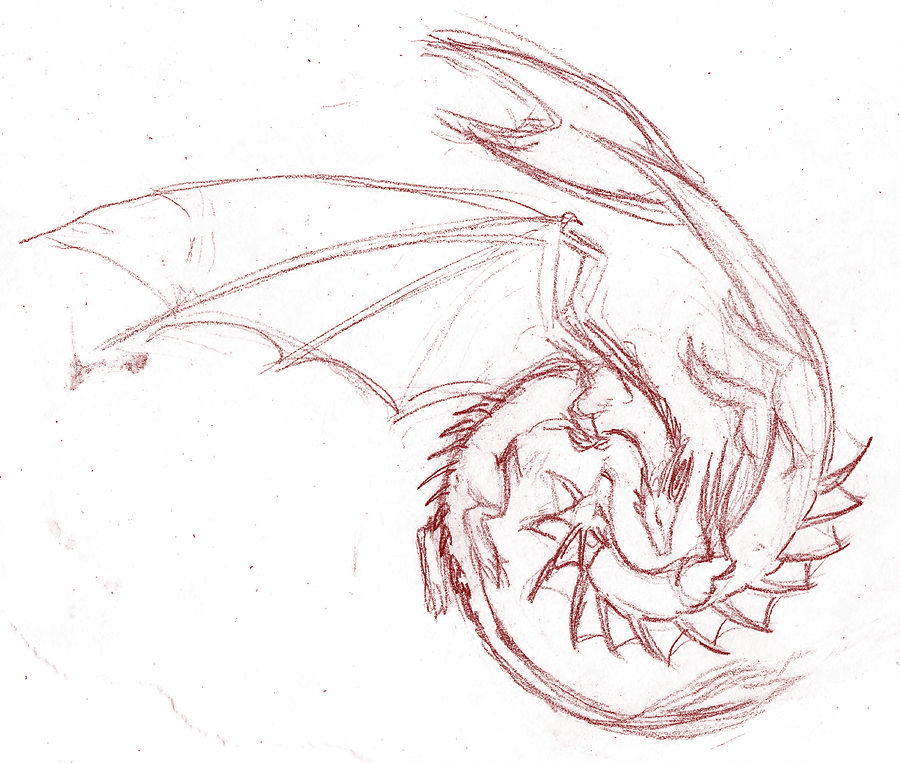
\includegraphics[width=\textwidth / 2 ]{img/drachen}
\end{figure}
